\documentclass[]{scrartcl}
\title{Vorlesung Analysis II}
\usepackage{amsmath,amssymb,amsfonts}
\usepackage{stmaryrd}
\usepackage{mathtools}
\usepackage{latexsym}
\usepackage{graphicx}
\usepackage{tikz}
\usepackage{xcolor}
\usepackage[most]{tcolorbox}
\usepackage{soul}
\usepackage{ upgreek }
\usepackage{hyperref}
\usepackage{tipa}
\usepackage[dvipsnames]{xcolor}
\hypersetup{
	colorlinks=true,
	linkcolor=blue,
	filecolor=magenta,      
	urlcolor=cyan,
	pdftitle={Overleaf Example},
	pdfpagemode=FullScreen,
}
\newcommand{\redcircle}[1]{%
	\tikz[baseline=(char.base)]{
		\node[shape=circle, draw=red, text=red, thick, inner sep=1pt] (char) 
		{\textbf{#1}};
	}%
}
\newcommand{\bluecircle}[1]{%
	\tikz[baseline=(char.base)]{
		\node[shape=circle, draw=blue, text=blue, thick, inner sep=1pt] (char) 
		{\textbf{#1}};
	}%
}
\newcommand{\blackcircle}[1]{%
	\tikz[baseline=(char.base)]{
		\node[shape=circle, draw=black, text=black, thick, inner sep=1pt] 
		(char) 
		{\textbf{#1}};
	}%
}
\newcommand{\orangecircle}[1]{%
	\tikz[baseline=(char.base)]{
		\node[shape=circle, draw=orange, text=orange, thick, inner sep=1pt] 
		(char) 
		{\textbf{#1}};
	}%
}
\newcommand{\redul}[1]{\setulcolor{red}{\ul{#1}}}
\newcommand{\blueul}[1]{\setulcolor{blue}{\ul{#1}}}
\newcommand{\yelul}[1]{\setulcolor{yellow}{\ul{#1}}}
\newcommand{\greenul}[1]{\setulcolor{green}{\ul{#1}}}
\newcommand{\oraul}[1]{\setulcolor{orange}{\ul{#1}}}
\setul{1pt}{3pt} % Linienhöhe und Abstand zum Text (optional anpassbar)

\setlength{\topmargin}{-.5in} \setlength{\textheight}{9.25in}
\setlength{\oddsidemargin}{0in} \setlength{\textwidth}{6.8in}
\setlength{\parindent}{0pt}

\begin{document}
	\maketitle
	\textbf{\underline{Teil 2: Topologische Grundbegriffe in metrischen Räumen}}\\
	\\
	\textbf{\underline{an13: Stetigkeit, Kompaktheit}}\\
	\\
	\textbf{\underline{\underline{Stichworte:} Stetigkeit, Bilder Kompakter mengen sind Kompakt, gleichmäßig stetig}}\\
	\\
	\textbf{\underline{Literatur:}} \blueul{[Forster], Kapitel 3}\\
	\\
	\textbf{13.1. \underline{Einleitung:}} Wir verallgemeinern den Stetigkeitsbegriff auf metrische Räume. Die grundlegenden Eigenschaften stetiger Abbildungen werden gezeigt. Die Bedeutung des Kompaktheitsbegriffs wird deutlich, u.a. in dem Satz, dass Bilder Kompakter mengen wieder Kompakt sind, als Verallg. des Satzes vom Min./Max.\\
	\\
	\textbf{13.2. \underline{Vereinbarung:}} Seien (R,S($\leftarrow$rho)), ($\rho,\sigma(\leftarrow $sigma)) metrische Räume, $f:R\rightarrow S.$\\
	\\
	\textbf{13.3. \underline{Def.:}} f heißt \redul{stetig in $a\in R$}:$\Leftrightarrow \forall \epsilon \textgreater0\exists \delta \textgreater 0 \forall x\in R: S(x,a)\textless \delta\Rightarrow\sigma(f(x),f(a))\textless\epsilon$.\\
	$\Leftrightarrow \forall V \in \mathcal{U}_{f(a)}\exists U \in \mathcal{U}_a:f(U)\subseteq V$.\\
	f heißt \redul{stetig (auf R)}: $\Leftrightarrow \forall a\in R:f$ stetig in a\\
	f heißt \redul{stetig in $D\subseteq (R,S)$}:$\Leftrightarrow f_{rD}$ stetig.\\
	\textopencorner dabei gilt: D $\subseteq (R,S) \Leftrightarrow (D,S_{rD\times D})$ metrischer Raum\textcorner\\
	\\
	\textbf{13.4. \underline{Bem.:}} f \greenul{in a stetig}$\Leftrightarrow$\greenul{$\forall x_k\rightarrow a: f(x_k) \rightarrow f(a)$}.\\
	\underline{Bew.:} "$\Leftrightarrow$": Gelte $x_k\rightarrow a, V\in\mathcal{U}_{f(a)}.$\\
	\oraul{Beh.:} Für fast alle k gilt $f(x_k) \subseteq V.$\\
	Denn: Nach Vor. $\exists U \in \mathcal{U}_a: f(U)\subseteq V (\OE U = B_a^\epsilon).$\\
	In $B_a^\epsilon$ liegen fast alle $x_k$, also liegen in V fast alle $f(x_k)$.\\
	Da v beliebig, folgt: $f(x_k)\rightarrow f(a).\\$
	"$\Leftarrow$": \oraul{Ann.:} f nicht stetig. \oraul{Konstruktion} : $\exists V \in \mathcal{U}_{f(a)}\forall U \in \mathcal{U}_a: f(U)\nsubseteq V$,\\
	\OE $U=B_a^{1/k}:\exists x_k \in B_a^{1/k}, f(x_k)\notin V\\
	x_k\rightarrow a$, aber $f(x_k)\nrightarrow f(a)$.\\
	\begin{figure}[h]
		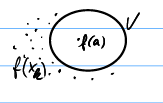
\includegraphics[width=3 cm,height=2cm]{bsp kap 13.4}
	\end{figure}\\ 
	\hfill$\square$\\
\end{document}